\chapter{A propos des interactions biotiques et des contraintes environnementales à l'échelle biogéographique}
\label{chap1}

\section{Résumé en français}
%
\subsection{Contexte scientfique}

En 1967, Robert MacArthur et Edward O. Wilson publient leur théorie de la
biogéographie des îles.
Comme mentionner dans l'introduction, la TIB demeurt le support de nombreux travaux de recherche,
ce dont témoigne le livre publié en 2010 et édité par Jonathan B. Losos et Robert E. Ricklefs~: \emph{The Theory of Island Biogeography Revisited} \citep{Losos2010}.
Ce livre souligne l'importance des travaux de MacArthur et Wilson et fait l'inventaire des questions qui restent à explorer.
Parmi ces interrogations, figurent celles relatives au rôle des relations trophiques, développées au sixième chapitre par Robert D. Holt.

C'est précisément sur ce sujet que portent les travaux de Dominique Gravel et ses collègues présentés dans l'article \emph{Trophic Theory of Island Biogeography} publié en 2011 dans \emph{Ecology Letters} \citep{Gravel2011}.
Dans cet article, les auteurs montrent comment les résultats de la TIB sont modifiés par la prise en compte des liens écologiques unissant proies et prédateurs.
Cet article est également le point de départ de mon premier article de thèse. L'objectif fixé était de 1- généraliser à tous types d'interaction le travail de Gravel et ses collègues
et 2- introduire les contraintes environnementales afin de comprendre dans quelle mesure les prédictions de la théorie classique en étaient affectées.

Pour y parvenir, la clef de mon travail a été de considérer les espèces non pas de manière indépendantes, mais comme des assemblages, des communautés possibles.
J'ai alors été capable de bâtir des probabilités de survie dépendantes de la configuration du réseau écologique présent sur l'île.
De même, les probabilités de colonisation des espèces du continent ont été reliées aux conditions environnementales de l'île.
Après avoir montré comment le modèle a été construit et donné des prédictions simples, je me suis intéressé à des réseaux de
10 espèces présentant des types d'interactions différents~: mutualisme, prédation et compétition, le long de gradients environnementaux.
Ce qui ressort des simulations est un portrait des impacts potentiels des interactions sur la distribution des espèces et la nécessité de les intégrer dans les SDMs.
Dépendamment de leur nature et de leur nombre, les interactions peuvent changer drastiquement la biodiversité attendue dans le cadre de la TIB.
Cela pourrait avoir des conséquences majeures sur nos prévisions de richesse spécifique dans le contexte actuel des changements globaux.
Le modèle développé dans ce chapitre est basé sur les chaînes de Markov, l'ensemble des aspects mathématiques de ce modèle sont présentés en détails à l'annexe \ref{annII}.
Certains des développements sont repris dans un article dont je suis co-auteur et dont je présente ma contribution à cet article à l'annexe \ref{annIII}.



\subsection{Publication associée}

Le travail réalisé a donné lieu à un article intitulé
\emph{On the integration of biotic interaction and environmental constraints at the biogeographical scale}
\citep{Cazelles2016a}. Il fut accepté pour publication à l'automne 2015 dans le
journal \emph{Ecography} et a été publié en ligne en décembre 2015.
Le DOI associé est: \textbf{10.1111/ecog.01714}.
La conception de l'article est le résultat de nombreux échanges entre l'ensemble des auteurs de l'article.
J'ai développé le modèle et l'ensemble des scripts pour aboutir aux résultats finaux.
Dominique Gravel a supervisé l'ensemble des étapes et est devenu le dernier auteur.
David Mouillot et Nicolas Mouquet ont grandement contribué à la rédaction du manuscrit.
Afin de promouvoir notre publication, j'ai également rédigé un article court sur le blog de la revue \emph{Ecography}
accessible en ligne à l'adresse suivante:
\url{http://www.ecography.org/blog/towards-integrated-theory-biogeography}.


\subsection{Traduction du résumé de l'article publié}

La biogéographie est concernée en premier lieu par la répartition spatiale de la
biodiversité dont elle produit les scénarios de variation dans un contexte de
changement environnemental. Les efforts déployés pour développer les modèles de
distribution d'espèces ont donné des outils qui, bien que prédictifs, sont
restés corrélatifs et ont largement ignorés les interactions biotiques.
Dans cet article, nous utilisons la théorie de la biogéographie des îles
en tant que première approximation d'une dynamique d'assemblage des communautés
locales dans un contexte de métacommunautés.Nous y superposons l'ensemble des
types d'interactions et nous introduisons les contraintes environnementales sur
la dynamique de colonisation et d'extinction. Nous développons une approche
probabiliste reposant sur les chaînes de Markov et nous calculons les
probabilités de réalisation des assemblages spécifiques plutôt que les
probabilités de présence des espèce une à une.
Nous considérons la distribution de richesse spécifique pour les différents
types d'interactions écologiques.
De plus, nous illustrons également le potentiel de notre approche en étudiant
l'articulation entre les différences de besoins écologiques, les interactions
et la distribution de la biodiversité le long d'un gradient environnemental.
Notre approche supporte l'idée que les recherches futures en biogéographie
requièrent une intégration cohérente de plusieurs concepts écologiques dans une
théorie unique afin de mener vers des innovations méthodologiques et
conceptuelles comme celui du changement des modèles de distributions espèce-centrés
vers des modèles communauté-centrés.


\emph{Les sections suivantes sont celles de l'article publié.}





\section{Title}

On the integration of biotic interaction and environmental constraints at the biogeographical scale.

\section{Authors}

Kévin Cazelles, Nicolas Mouquet, David Mouillot, Dominique Gravel.


\section{Abstract}

Biogeography is primarily concerned with the spatial distribution of biodiversity, including performing scenarios in a changing environment. The efforts deployed to develop species distribution models have resulted in predictive tools, but have mostly remained correlative and have largely ignored biotic interactions. Here we build upon the theory of island biogeography as a first approximation to the assembly dynamics of local communities embedded within a metacommunity context. We include all types of interactions and introduce environmental constraints on colonization and extinction dynamics. We develop a probabilistic framework based on Markov chains and derive probabilities for the realization of species assemblages, rather than single species occurrences. We consider the expected distribution of species richness under different types of ecological interactions. We also illustrate the potential of our framework by studying the interplay between different ecological requirements, interactions and the distribution of biodiversity along an environmental gradient. Our framework supports the idea that the future research in biogeography requires a coherent integration of several ecological concepts into a single theory in order to perform conceptual and methodological innovations, such as the switch from single-species distribution to community distribution.


\section{Introduction}

Biogeography is concerned with the description of the distribution of biodiversity and understanding its underlying processes. The discipline is central to the simulation of future scenarios of biodiversity under climate change \citep{Thuiller2013}. The extensive development of statistical models of species distributions based on actual ranges and environmental data have provided valuable knowledge and predictions \citep{Kearney2004}, but often remain purely correlative. There is now consensus that future developments in biogeography will require solving critical limitations of species distribution models \citep{Kissling2012} and incorporating explicitly biotic interactions and dispersal \citep{Lavergne2010}. This effort must be supported by theory in order to guide model development, maintain tractability and manage complexity. Developing a mechanistic theory of species distribution will require an integration of three fundamental principles and their interplay \citep{Thuiller2013}: 1) how local and regional dynamics are linked, 2) how species interact with the abiotic environment and 3) how they are embedded in a network of biotic interactions. Each of these principles are discussed in detail below.

A cornerstone of biogeography is the recognition of the contribution of regional-scale processes such as disturbances, historical contingencies (e.g. macro evolutionary history or glaciations) and dispersal limitations to local community dynamics \citep{Ricklefs1987}. The metacommunity concept has been proposed as a simple framework to link different spatial scales in ecology \citep{Leibold2004}. It emphasizes reciprocal feedbacks between local scale processes, such as competitive interactions and local adaptation, and regional scale processes such as dispersal, gene flow, and speciation. A central concept of metacommunity ecology is the idea that local communities are highly dynamic owing to colonization events and local interaction, resulting in a spatial mosaic of assemblages sampled non-randomly from the regional species pool. As the concept matures there are new themes emerging, such as the investigation of evolution in metacommunities \citep{Urban2008}, and spatial food webs \citep{Massol2011,Gravel2011}. The field provides remarkable concepts and tools to build an integrated theory for biogeography.

Species distribution is also constrained by physiological requirements, which is at the core of the niche concept \citep{Peterson2011}. The niche is usually defined as a N-dimensional environmental and resource hyper-volume within which a species is able to maintain a viable population over the long term \citep{Chase2003}. Recent developments refined this definition based on demography and metapopulation dynamics \citep{Holt2009}. The abiotic niche, often referred as the Grinnelian niche, has been central to the development of species distribution models \citep[SDMs,][]{Jeschke2008}. Despite all of its criticisms, SDMs remain remarkably popular and operational for conservation ecology \citep{Guisan2013}. Recent attempts to improve the quantification of the niche include the addition of experimental assessments of the fundamental physiological constraints, as well as dispersal and proxies of biotic interactions \citep{Boulangeat2012}. The search for the most adequate set of environmental variables explaining diversity should be continued despite criticisms of the actual SDMs, and most of all must constitute a central principle of a general theory for biogeography.

Finally, species are not isolated, they are embedded within complex networks of ecological interactions. While interactions define community ecology, they are less informative for biogeography \citep{Peterson2003}. Theory predicts that interactions in small community modules (2-4 species) should influence range limits \citep{Gilman2010}, but there is no extension to highly diverse communities. It has been hypothesized that factors determining distribution are hierarchical, such that climate would govern the distribution at the regional scale while biotic interactions would be more important at the local scale \citep{Araujo2014}. However an increasing number of studies emphasizes the role of local interactions as a major factor influencing geographical ranges \citep{Jabot2012, Gotelli2010}. The representation of interactions in a network is a convenient method to summarize the type and strength of interactions among species, their organization \citep{Proulx2005} and their consequences on dynamics \citep{Allesina2012a}. Food webs were first considered in the development of a trophic theory of biogeography \citep{Gravel2011}, where it was shown that a diversity of interactions enhance persistence. Networks are however more than food webs and are rarely made of a single type of interaction \citep{Kefi2012}. Mutualism, competition and indirect effects \citep{Wootton1994}, for instance, also impact local environmental suitability \citep{Godsoe2012}. Tools and knowledge acquired through the study of local ecological networks, such as the community matrix and metrics of structure \citep{Allesina2012a}, must now be incorporated into a theory for biogeography.

These three principles should be all mixed together to provide an integrated assessment of their relative contribution to species distribution. To do so, the theory of Island Biogeography (hereafter referred as TIB) \citep{MacArthur1967, Warren2015} is a convenient starting point. The TIB describes variations of species richness among islands as a dynamic equilibrium between two opposite processes, colonization and extinction, directly linked with island characteristics. The TIB is a metaphor that goes beyond the intrinsic interest of islands; it serves as a first approximation to understanding the assembly of local communities embedded in a metacommunity context with straightforward species flux. The simplicity of the model and the relevance of its predictions demonstrate after more than 50 years since its publication it is still a useful tool in ecology and conservation \citep{Cook2002, Warren2015}. The TIB emphasizes the role of regional processes to local community assembly. Indeed it can be regarded as the simplest representation of metacommunity dynamics \citep{Leibold2004}. Furthermore, the model is easily expandable. Following \cite{Holt2009}, \cite{Gravel2011} introduced trophic interactions in the TIB (hereafter the trophic TIB, TTIB;). Species interactions were found to be a key factor to understand species distributions, as the probability of finding any species in a locality increases with the generality of its diet and decreases with trophic rank.

We propose to generalizes of the TIB by integrating the three principles described above. The TIB already explicitly includes the effect of regional processes (colonization and extinction dynamics) on local community assembly, and the TTIB includes predator-prey interactions. We extend this framework to all potential interactions, thus resulting in a general model of metacommunity dynamics, akin to the Lotka-Volterra equations for local community dynamics. We also incorporate abiotic constraints on colonization and extinction dynamics. Hence we integrate the ingredients we believe are essential to model biodiversity distribution at the biogeographical scale. With this model in hand we then describe species distribution along environmental gradients. We use the mathematical formalism of Markov Chains \citep{kemeny1983finite, Black2012} to derive expected assemblages and co-distribution at both the local and the regional scale. We illustrate how the interplay between biotic interactions and environmental requirements can affect the distribution of biodiversity over environmental gradients. Our results support the idea that the future research in biogeography require a consistent integration of several ecological concepts into a single framework to build promising approaches such as the switch from single-species distributions to community distributions.

\section{The model}

%--------------------------------------------------------------
\subsection{A simple probabilistic biogeographical model}

The challenge of adding species interactions within the classical model of the TIB is gaining generality without losing simplicity. Following MacArthur and Wilson's theory, we model the dynamics of occurrence probability of a species $i$ in a local community. Species occurrence is the result of a balance between colonization and extinction dynamics, which occur at rates $c_i$ and $e_i$ respectively,. Local species richness is given by the sum of occurrence probabilities over all species of the regional species pool $P$, here simply defined as the set of all species whose propagules \citep[as defined in][]{Simberloff1969} can land on the island considered. The model thereby takes into account local (extinction) and regional (colonization) processes. More precisely, the dynamics of occurrence probability of species i, $p_i$, follows:
%-------------
\begin{eqnarray}
\label{chap1eq1} \frac{dp_{i}}{dt}&=&c_i(1-p_{i})-e_ip_{i}
\end{eqnarray}
%-------------
Here, $c_i$ and $e_i$ are constant and a property of species $i$. In this widespread version of the TIB, also called the linear version of the TIB \citep{Schoener2010}, the equilibrium occurrence probability of a species $i$ is given by $p_{i,eq}=\frac{c_i}{e_i+c_i}$. Also, species are assumed to be independent, therefore, the richness $S_{eq}$ is given by the sum of the $P$ different $p_{i,eq}$. The linear TIB can be modified to include trophic interactions \citep[after][]{Gravel2011} and we propose to extend it to all types of interactions. To reach that goal, the first step is to find a way to derive the expected species composition at any time. This composition can actually be depicted at any time by a vector of $P$ zeroes and ones indicating, respectively, presences and absences of each species considered, these combinations will be referred as assemblages. Following Mac-Arthur and Wilson, we use a stochastic modelling approach to describe the dynamics of assemblages. The simplest scenario is the one species case. Here there are only two assemblages for the locality: one with species $i$ present and the other without. Let $X_{i}$ be a random variable describing the occurrence of species $i$. When species $i$ is present in the locality, $X_i$ is 1, when it is absent $X_i$ is 0; $X_i$ is then a Bernoulli variable.
We define this random variable at any time $t$ which describes a stochastic process we denote $\mathbf{X_{i,t>0}}$. The occurrence probability of species $i$ at time $t+dt$ ($dt$ being a very small time step) is then given as follows:
%-------------
\begin{eqnarray}
\nonumber \mathbb{P}(X_{i,t+dt}=1) &=& \mathbb{P}(X_{i,t+dt}=1|X_{i,t}=1)\mathbb{P}(X_{i,t}=1) \\
\label{chap1eq2} & & +\mathbb{P}(X_{i,t+dt}=1|X_{i,t}=0)\mathbb{P}(X_{i,t}=0)
\end{eqnarray}
%-------------
$\mathbb{P}(X_{i,t+dt}|X_{i,t})$ is the conditional probability describing $X_{i,t+dt}$ stating $X_{i,t}$. As $X_{i,t+dt}$ solely depends on $X_{i,t}$ (not on other earlier time steps) we have a discrete-time Markov chain. In this process, species $i$ will be present in a locality at time $t+dt$ if it was already present at time $t$ and persisted (meaning it did not go extinct, with probability $(1-e_idt)$, or if it was absent and colonized the community from the mainland (with probability $c_idt$). Note that $dt$ is small enough to get $0<c_idt<1$ and $0<e_idt<1$. Hence, equation~\eqref{chap1eq2} becomes:
%-------------
\begin{equation}
\label{chap1eq3} \mathbb{P}(X_{i,t+dt}=1)=c_idt\mathbb{P}(X_{i,t}=0)+(1-e_idt)\mathbb{P}(X_{i,t}=1)
\end{equation}
%-------------
This equation leads to \eqref{chap1eq1} when $dt$ tends to zero. This formulation keeps the simplicity of the original MacArthur and Wilson model, but can also more generally be used to consider the probability of any given assemblage. $\mathbb{P}(X_{i,t+dt}|X_{i,t})$ defines the rules to switch from one assemblage to one another during the interval $dt$.
There are $P$ occurrence probabilities we gather within $\mathbf{Y_{t>0}}=(\mathbf{X_{1,t>0}}, \mathbf{X_{2,t>0}}, ..., \mathbf{X_{P,t>0}})$ which leads to the description of $2^P$ assemblages depicted by a given collection of zeros and ones.
The conditional probabilities provide the transition from one local assemblage $k$ to any other $l$ during $dt$. For any species $i$ there are only four possible cases: at time $t$ either species $i$ is locally absent and colonizes the locality ($I_1$) or not ($I_2$) during $dt$, either species $i$ is present and goes extinct ($I_3$) or survives ($I_4$) during $dt$. The conditional probabilities between two communities states ($l$ and $k$) can then be simply derived from these four probabilities:
%-------------
\begin{eqnarray}
 \nonumber \mathbb{P}(\mathbf{Y_{t+dt}}=\text{"state k"}| \mathbf{Y_{t}}=\text{"state l"}) &=& \prod_{\substack{i_1\in I_1}}c_{i_1}dt\prod_{\substack{i_2\in I_2}}(1-c_{i_2}dt)
\\  \label{chap1eq4} & &~~\prod_{\substack{i_3\in I_3}}e_{i_3}dt\prod_{\substack{i_4\in I_4}}(1-e_{i_4}dt)
\end{eqnarray}
%-------------
We now apply the complete probability formula as defined in \eqref{chap1eq2} to get the probability of observing one assemblage at $t+dt$ given its state at $t$. This is where the main benefit of Markov chain models is: it allows us to derivate exact solutions for the probabilities for assemblages, instead of a set of independent occurrence probabilities for each species. This approach is promising for building joint species distribution models (see Discussion). This property will be fully explored in the next section to include interactions.

Consider as an example a pool of two species ($P=2$) for which we find four assemblages: at any time $t$, a locality can contain either two species $(X_{1,t}=1, X_{2,t}=1)$, only one species $(X_{1,t}=1, X_{2,t}=0)$ and $(X_{1,t}=0, X_{2,t}=1)$, or none of them $(X_{1,t}=0, X_2=0)$. The transition from one local assemblage to another is then easily obtained. Table \ref{tb1} presents these conditional probabilities (application of \eqref{chap1eq4}). This is actually the transition matrix of a Markov chain we solve (by calculating one eigen value, see below). To illustrate the dynamics expected in TIB from our assemblage point of view, we simulate the model as follows: $c_1=c_2=0.15$, $e_1=e_2=0.05$, $\mathbb{P}(X_{1,0}=0, X_{2,0}=0)=0.6$ and $\mathbb{P}(X_{1,0}=1, X_{2,0}=0)=0.4$, so species $2$ is absent at time $t=0$.
Just as for the single species situation, the probabilities of observing each community tend to an equilibrium (Fig.\ref{chap1fig1}, panel A). By summing the previous probabilities where a given species (1 or 2) is present (the conditional probabilities) we get its overall occurrence probability (marginal probability, Fig.\ref{chap1fig1}-B). Finally, we can calculate the expected number of species in a locality (Fig.\ref{chap1fig1}-C), in agreement with the TIB. Interestingly, this calculation is often achieved in the other way. Firstly, the presence probability of all species are computed: $\mathbb{P}(X_i)=\frac{c_i}{c_i+e_i}$. Then the richness is obtained under the assumption that species are independent and so $P(X_i,X_j)=\mathbb{P}(X_i)\mathbb{P}(X_j)$. We show below that occurrence probabilities of each assemblage is a key to introduce interactions among species.


%--------------------------------------------------------------
\subsection{Integrating biotic interactions}

We start by representing the interaction network by a community matrix $\mathbf{A}$ of $P$ species that we incorporate into the Markovian TIB chain model. The elements $\alpha_{i,j}$ of $\mathbf{A}$ quantify the effect of species $j$ on the dynamics of species $i$. We first consider that interactions could alter both the colonization and the extinction probabilities \citep{Gravel2011}. When $\alpha_{i,j}$ is negative, the colonization probability of species $i$ decreases and/or its extinction probability increases when $j$ is found locally. Inversely, when $\alpha_{i,j}$ is positive, the colonization probability increases and/or the extinction probability decreases. Note that diagonal elements provide the extinction probability per time unit when no other species is present.

\begin{table}[h!]
\centering
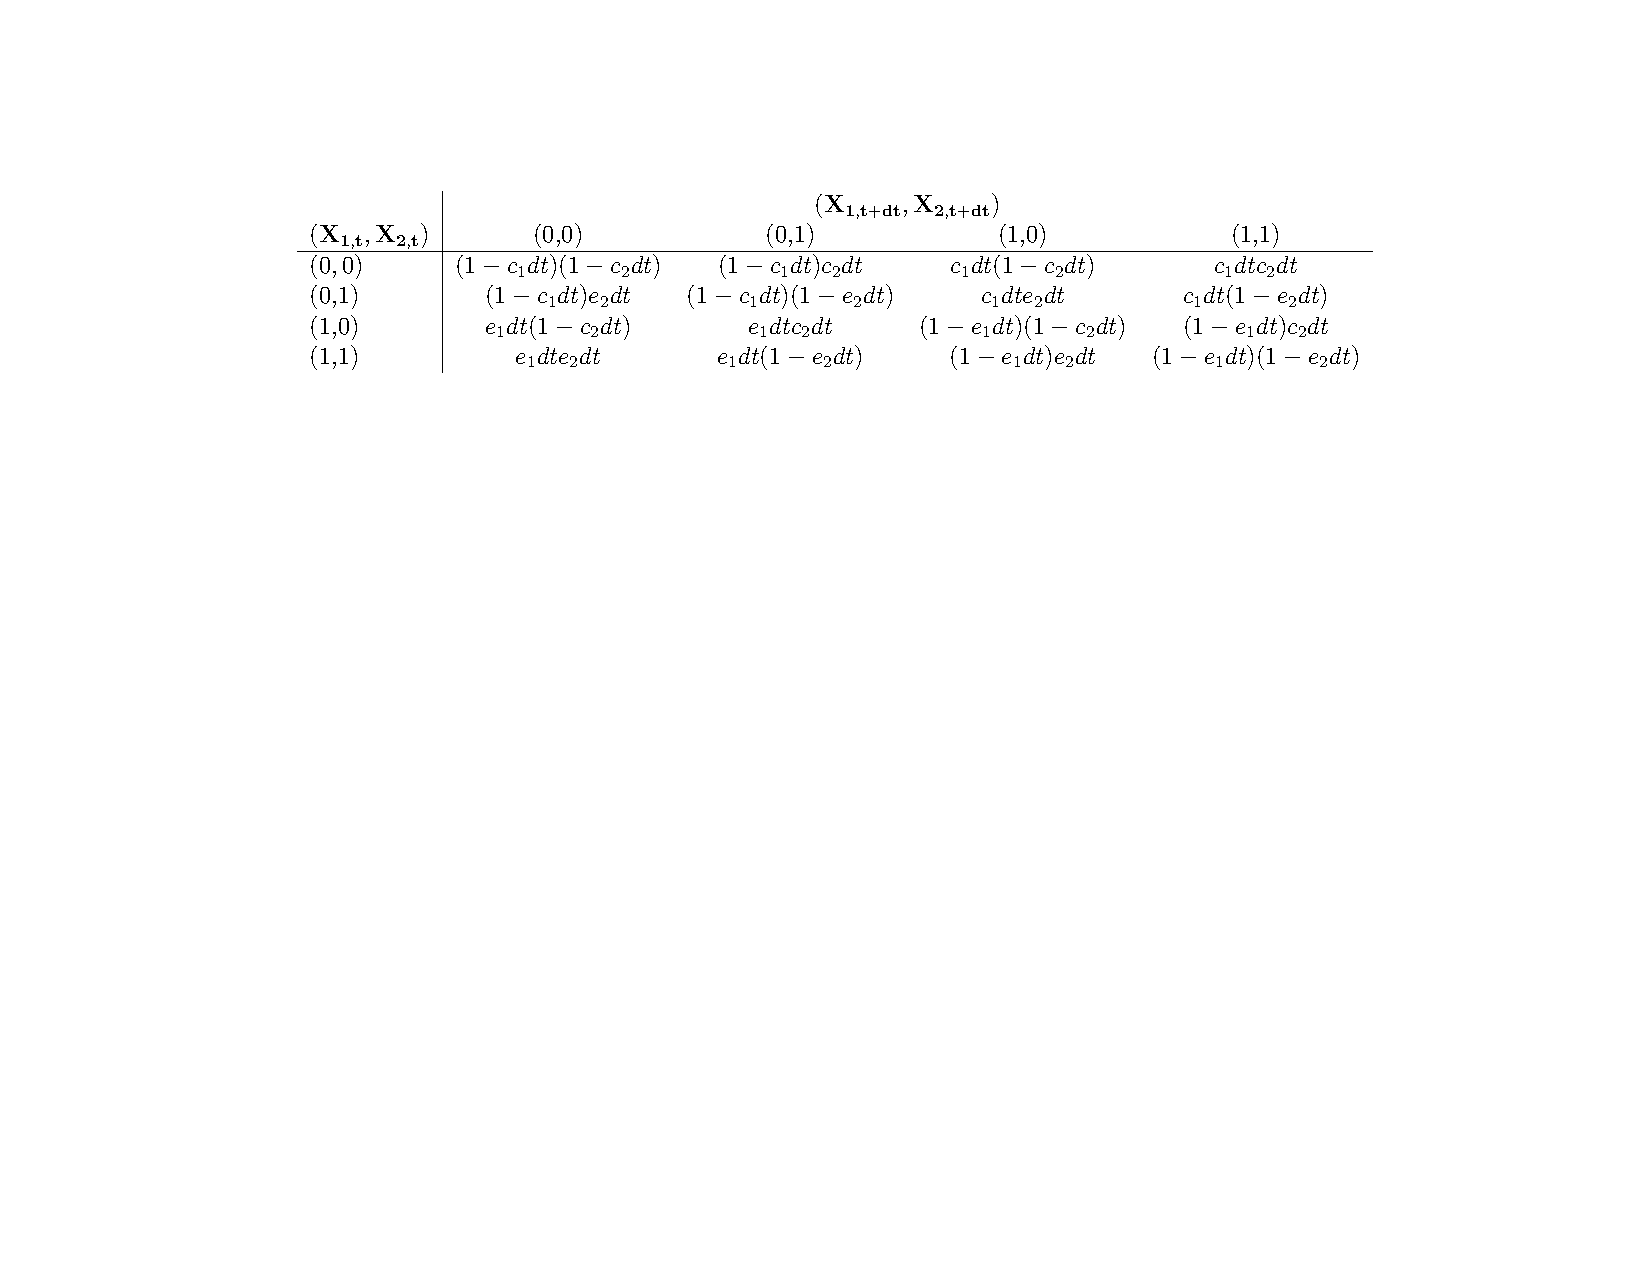
\includegraphics[scale=0.85]{./chapitre1/table1.pdf}
\caption[Conditional probabilities between potential assemblages]{\textbf{Conditional probabilities between potential assemblages}. At any time $t$ we calculate all the possible conditional probabilities between the four potential assemblages for a two species regional pool. These probabilities are derived by multiplying probabilities of single species events defined in equation~\eqref{chap1eq4}. By doing so, we build the transition matirx of our markov chain where species are assumed to be independent. We release this hypothesis by linking extinction coefficients and species assemblages.}
\label{tb1}
\end{table}

The elements of the community matrix $\mathbf{A}$ represent the pairwise effects of ecological interactions on transition probabilities. To account for the cumulative effects of local interactions on transition probabilities, we make colonization and extinction probabilities community dependent. As explained above, at a time $t$, the $\mathbf{Y_t}$ vector gives the local assemblages. We calculate the sum of interactions at any time and for each species as $\mathbf{v}=\mathbf{A}\mathbf{Y_t}^T$ (where $^T$ denotes the transpose operator). Our approach can be interpreted as a spatial analogue to the generalized Lotka-Volterra model because it takes into account the impact of the whole network of interactions on each species dynamics and can deal with any type of interaction. We denote the coefficients of $\mathbf{v}$ by $v_i$, they are species-specific parameters (weighted by parameter $d_i$) of two species-specific functions: $f_i$ and $g_i$, respectively, standing for extinction and colonization probabilities for species $i$. Note that at this stage we do not define any specific function relating interactions to colonization ($f_i$) and extinction probabilities ($g_i$), to keep the description of the model general (see below for some proposed functions). At each time step, the local community composition impacts: i) the colonization probability of species present in the regional pool but absent from the local community, and ii) the extinction probability of species present on the local community.

If we expand the two species example (labelled $1$ and $2$, Table \ref{tb1}), according to the general model, we define two $f$ functions ($f_1$ and $f_2$) linking interaction and extinction and two $g$ functions linking extinction and colonization ($g_1$, $g_2$). At this stage, to reduce the model's complexity, we consider that interactions solely impact extinction probabilities. This assumption is reasonable if we consider that local interactions impact mostly demography (possibly leading to extinction) and that colonization success solely depends on the first propagule (interactions occur after arrivals). Therefore $g_1$ and $g_2$ are constant functions, respectively,, returning $c_1$ and $c_2$. The functions $f$ are assumed to have a sigmoid shape \eqref{chap1eq5}. There are many reasons such a function is of interest: 1) we get a clear link with the basic extinction probability, i.e. $e_i$ for an interaction strength of 0; 2) we define both a minimum and a maximum extinction probability; 3) the first interactions to occur are the most influential (\cite{Gravel2011} considered that at least one interaction was required to persist, which is very similar).
%-------------
\begin{eqnarray}
\nonumber f_i(\mathbf{v})&=&f(\mathbf{v},(e_i,e_{i,min},e_{i,max},d_i)) \\
\label{chap1eq5} &=&e_{i,min}+\frac{1}{\frac{1}{e_{i,max}-e_{i,min}}+\left(\frac{1}{e_{i}-e_{i,min}}-\frac{1}{e_{i,max}-e_{i,min}}\right) \exp(d_i*v_i)}  \\
g_i(\mathbf{v})&=&c_i
\end{eqnarray}
%-------------
To illustrate how interactions modify occurrence probabilities, we simulate the model for two networks: $A_1$ where all interactions are negative and $A_2$ where they are all positive. We consider null diagonal elements for both networks. Consequently, there is no difference with the model without interaction when one species is alone in the locality. Simulation results are presented at Figure \ref{chap1fig2}. Panel A presents the functions $f_1$ and $f_2$ we chose for our two species example. For networks $A_1$ and $A_2$, we show how interactions alter the probabilities of observing different assemblages (respectively, Fig.\ref{chap1fig2}-B and Fig.\ref{chap1fig2}-C). The assemblage with both species present (solid red lines) is the most affected by interactions, switching from an occurrence probability of 0.2 (for negative interactions) to 0.8 (for positive interactions). Positive interactions enhance, as expected, co-occurrence while negative interactions prevent species from being found on the same island. Consequently, occurrence probabilities of single species states are lower in $A_2$ than in $A_1$. According to a defined network, occurrence probabilities of the different assemblages are then modified, which affect the expected species richness (Fig.\ref{chap1fig2}-D).

\begin{figure}[h!]
\centering
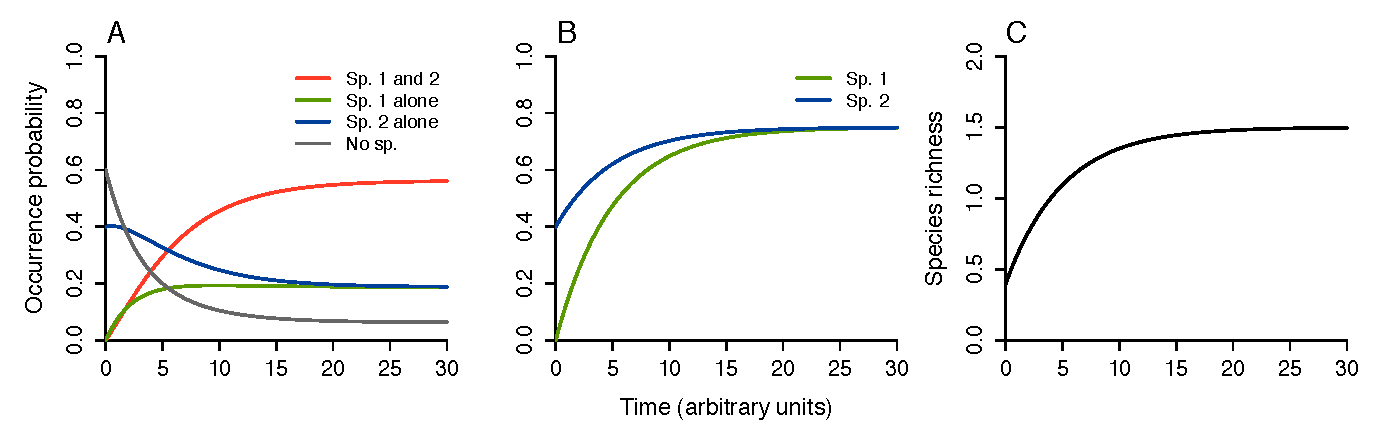
\includegraphics[width=\textwidth]{./chapitre1/fig1.eps}
\caption[Dynamics of the community assembly]{\textbf{Dynamics of the community assembly}. As a direct development of MacArthur and Wilson model, we simulate for two species, the dynamics of the four communities states with different initial conditions associated (A). By summing every states where one given species is present we get the occurrence probability of two considered species (B). Finally by summing the four states probabilities weighted by their species richness, we get the classical model of MacArthur and Wilson (C). The calculation of (B) and (C) does not require species being independent while classical approaches focus on (B) to derive (A) and (C) under this assumption of independence.}
\label{chap1fig1}
\end{figure}





%--------------------------------------------------------------
\subsection{Integrating environmental gradients}

We now introduce the effect of abiotic conditions, such as climatic variables, on transition probabilities. We denote the vector of $n$ environmental conditions by $\mathbf{w}$: $\mathbf{w}=(w_1,w_2,...w_n)$. We first assume that physiological constraints can affect both colonization and extinction probabilities through the functions $f_i$ and $g_i$ (affecting, respectively,, extinction and colonization rates). Again the model in its general formulation does not presume any shape for these functions. We now have all the ingredients of an integrated model of biogeography as the transition probabilities at a location depend on 1) species-specific colonization and existence probabilities, 2) the network of interactions, 3) local community composition, and 4) local environmental conditions. In the general formulation of the model, functions $f_i$ and $g_i$ are functions of multiple variables ($\mathbf{v}$ and $\mathbf{w}$).

At any time $t$, for a regional pool of $P$ species among which interactions are summarized by the community matrix $\mathbf{A}$, in an environment characterized by $\mathbf{w}$, we can derive all transition probabilities. These constitute a transition matrix of a Markov chain that we denote $\mathbf{M}(\mathbf{v,w})$. Its elements, $\mu_{k,l}(\mathbf{v,w})$, give the probability the locality in assemblage $k$ turns into assemblage $l$ (left side of equation \eqref{chap1eq4}):
%-------------
\begin{eqnarray}
\nonumber \mu_{k,l}(\mathbf{w,v}) &=& \prod_{\substack{i_1\in I_1}}g_{i_1}(\mathbf{v}, \mathbf{w})dt \prod_{\substack{i_2\in I_2}}(1-g_{i_2}(\mathbf{v}, \mathbf{w})dt) \\
\label{chap1eq6} & & ~~ \prod_{\substack{i_3\in I_3}}f_{i_3}(\mathbf{v}, \mathbf{w})dt \prod_{\substack{i_4\in I_4}}(1-f_{i_4}(\mathbf{v}, \mathbf{w})dt)
\end{eqnarray}
%-------------
Note that the dimension of $\mathbf{M}(\mathbf{w})$ will increase as a power of the number of species $P$ and thus can rapidly becomes large. Let $\mathbf{C_t}$ be the line vector of the probability of observing each assemblage, defined by: $\mathbf{C_t}=\big(\mathbb{P}(\mathbf{Y_t}="\text{state }1"), \mathbb{P}(\mathbf{Y_t}="\text{state }2"),..., \mathbb{P}(\mathbf{Y_t}="\text{state }2^P")\big)$. The Markov Chain formalism defines the probability of the future community composition at time $t+dt$ as $ \mathbf{C_{t+dt}}=\mathbf{C_t}\mathbf{M}$. $\mathbf{C_t}$ asymptotically reaches the $\mathbf{C_{eq}}$ after a certain number of time steps. $\mathbf{C_{eq}}$ is given by the normalized left eigenvector associated to the first left eigenvalue.
%-------------
\begin{equation}
\label{chap1eq7}
\lim\limits_{\substack{l \to +\infty \\ l \in \mathbb{N}}} \mathbf{C_0}\mathbf{M}^l=\mathbf{C_{eq}}
\end{equation}
%-------------
$\mathbf{C_{eq}}$ contains the probability of all assemblages at the equilibrium. The occurrence probability of a given species, is provided by the sum of all probabilities of assemblage where that species is present. The richness at the equilibrium $S_{eq}$ is the sum of $\mathbf{C_{eq}}$ elements weighted by the number of species found in the associated assemblages.

For the sake of illustration, we further reduce the complexity of our model. We have previously removed the interactions ($\mathbf{v}$) from colonization ($g$) functions; we now state that extinction does not depend on environmental variables and so we remove the abiotic environment ($\mathbf{w}$) from extinction functions ($f$). This can be interpreted as the effects of the abiotic environment on extinction rate being included within $e_i$ (i.e. extinction rate without interaction). Furthermore, we assume solely one environmental variable and a Gaussian shape for $g_i$ functions \eqref{chap1eq8}. A simple function with a clear optimum and very low colonization for extreme environment values is.
%-------------
\begin{eqnarray}
\label{chap1eq8} g_i(w_1)=g(w_1,(c_i,h_i,r_i))&=&c_i*exp\left(- \left( \frac{w_1-h_i}{r_i} \right) ^2\right)
\end{eqnarray}
%-------------
This enables us to define an environmental optimum ($h_i$), a colonization probability per time unit ($c_i$) and also suitable range ($r_i$) for each species. Figure \ref{chap1fig3} presents the interplay between the three components of the integrated biogeographical model. The chosen functions for the environment-colonization relationship are illustrated in Panel A. For the two previous networks ($A_1$ and $ A_2$; illustrated in Fig \ref{chap1fig2}) we now compute the probabilities of observing the different assemblages at equilibrium, along the environmental gradient (Panel B and C). When interactions are negative (network $A_1$), species repulse each other and rarely co-occur, whatever the environment is. Most of their occurrence follow their abiotic niche (blue and green lines) as they are barely found together. Inversely, when interactions are positive (for $A_2$ network) they often co-occur where their abiotic niches overlap, thereby decreasing the probability of an empty community (Panel D, solid grey line). Finally, we present how interactions modify the resulting community composition along the environmental gradient (Panel D). Species richness is constrained by the distribution of abiotic niches and the sign of the interactions. As expected, the role of interactions is strongest when abiotic niches largely overlap.

%-------------------------
\begin{figure}[h!]
\centering
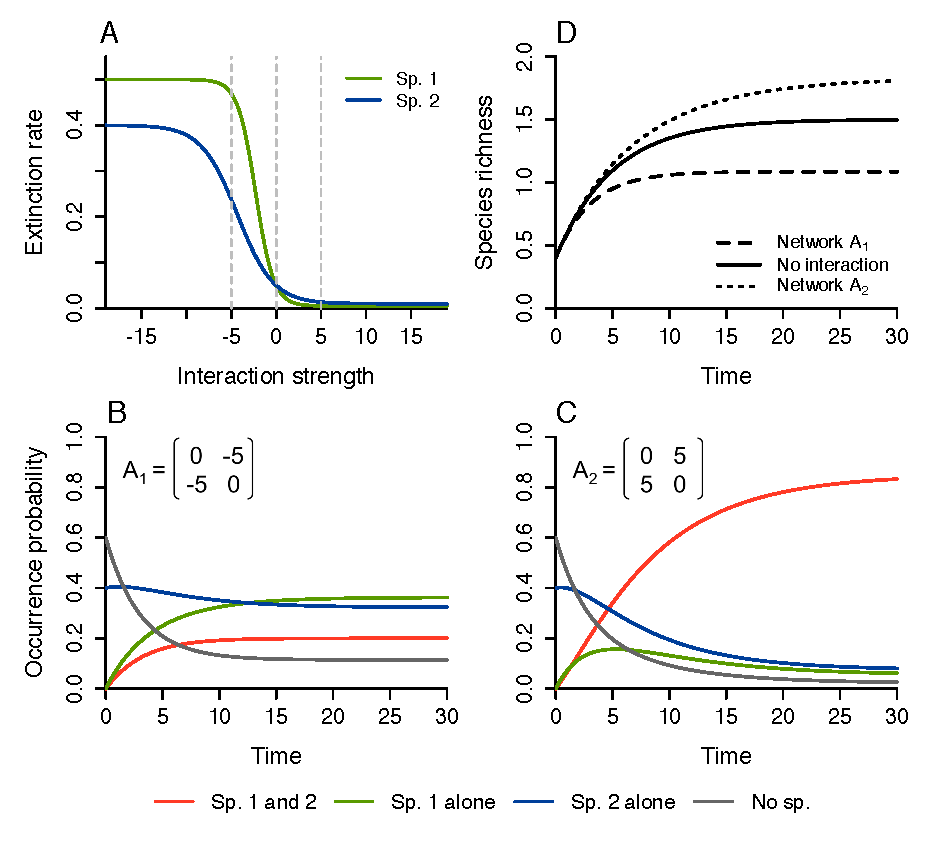
\includegraphics[width=\textwidth]{./chapitre1/fig2.eps}
\caption[Effects of biotic interactions on colonization-extinction dynamics]{\textbf{Effects of biotic interactions on colonization-extinction dynamics}. For any species $i$, the extinction probability $e_i$ is related to the strength of the interaction as shown in (A). The intersections of extinction curves with the grey dotted lines indicate the potential values of $e_i$ according to the different biotic context ($A_1$, $A_2$ and without interaction). We set the other parameters as follows: $c_1=c_2=0.15$, $\mathbb{P}(X_{1,0}=1 , X_{2,0}=0)=0.4$, $\mathbb{P}(X_{1,0}=0 , X_{2,0}=0)=0.6$, $\mathbb{P}(X_{1,0}=0 , X_{2,0}=1)=\mathbb{P}(X_{1,0}=1 , X_{1,0}=1)=0$. We then simulate the model for two simple networks $A_1$ and $A_2$ and present community assembly dynamics associated ((B) and (C)). Finally we compare the expected species richness on the locality (D) for our two networks and for the case without interaction which corresponds to the widespread linear version of the TIB.}
\label{chap1fig2}
\end{figure}

%--------------------------------------------------------------
%--------------------------------------------------------------
\section{Exploring the model}

In our exploration, we choose a regional pool $P$ of 10 species to keep the number of assemblages reasonable ($2^{10}=1024$) and to numerically compute the exact solution of the equilibrium distribution $\mathbf{C_{eq}}$. We consider four types of interaction matrices $\mathbf{A}$. The first situation corresponds to the classical MacArthur and Wilson model, where the $\mathbf{A}$ matrix is null (no interactions). For the three other scenarios we generate random matrices with fixed connectance (number of existing links divided by the number of potential links). The coefficients within $\mathbf{A}$ are drawn uniformly within $[0,1]$ and the sign of the interaction is determined by the action of one species on another, for instance, a predator has a negative impact on its prey leading to a negative $\alpha$ coefficient; in return, a prey has a positive effect on its predators. The intensity of the interaction is then determined by the $d$ coefficient of extinction functions (see equation~\eqref{chap1eq7}). We assume that the distribution of the links are given by the niche model \citep{Williams2000}. This model is simple and provides relevant random food webs with the same number of positive and negative interactions. For the two last scenarios, we keep the rules to distribute the links, but turn all the coefficients in $\mathbf{A}$ positive to generate a mutualism network, or negative for competition networks. Although these basic structures with exclusive interaction types are not realistic, they facilitate comparison among results. Hence, the scenarios simply differ by the sign distribution within the matrix $\mathbf{A}$:
(i) no interaction $\mathbf{A}$ is null, (ii) predation mixes both signs ``+/-'', (iii) mutualism only ``+'', (iv)- competition, only ``-''. With these scenarios in hands, we 1) present the assemblages probabilities associated with a given level of species richness and 2) we look at the species richness expected along an environmental gradient. For all figures presented hereafter we used 1000 randomly-generated $\mathbf{A}$ matrices.

%--------------------------------------------------------------
\subsection*{Assemblage probabilities}

First, we illustrate how interactions affect richness of species assemblages. To do so, we build the Markov chains for all the 1000 $\mathbf{A}$ matrices generated (connectance set to 0.2) and we calculate the vector $\mathbf{C_{eq}}$. This is a vector of 1024 occurrence probabilities (as we consider 10 species). Then we sum all the probabilities that correspond to assemblages of the same richness. We do so for three values of $d$ coefficient (0.1, 1 and 10); that is, we look at how the strength of interaction affect community richness predictions. Figure \ref{chap1fig4} presents the results of such investigation, with Panels A to C corresponding to the results for the three different values of the $d$ parameter.

As expected, positive interactions increase local species richness by diminishing extinction probabilities, while negative interactions weaken large communities (see the contrast between blue and red symbols on Fig.\ref{chap1fig4}). This is stressed as interaction strengths increase, that is for increasing values of $d$. Indeed, when $d$ is low, there is almost no difference among scenarios because interactions do not impact strongly colonization and extinction dynamics; occurring species can be regarded as mostly independent. All scenarios converge to the classical TIB scenario (no-interaction, grey symbols), the resulting species richness distribution is binomial (here for all species $p_{i,eq}=0.5$ as $c_i=e_i=10^{-5}$). Differences between interaction types increase with $d$. Species rich mutualistic communities are more likely to occur since positive interactions tends to promote co-occurrence. Therefore species occurrence can be dramatically affected by the strngth of interactions: for $d=10$ (Panel C in Fig. \ref{chap1fig4}), the species richness is 9.46 for positive interactions (red symbols), 2.24 for the negative ones (blue symbols) and 5 without interactions. When positive and negative interactions are mixed (our predation scenario, green symbols on Fig.\ref{chap1fig4}), it seems that the negative effect of predators on their prey prevails and so predation reduces species richness, but less than for competitive networks.

As we introduce variability through the use of randomly-generated matrices, we also compute the standard deviation associated with occurrence probabilities. The variability is provided as the coloured vertical bars found in Fig. \ref{chap1fig4} which stand for 50\% of the total standard deviation. Clearly, variability increases with (i) the strength of interaction and (ii) the occurrence probability. Although this can simply reflect the variability of values found in $\mathbf{A}$ matrices, this could potentially be caused by the variability of the location of non-zero values in  $\mathbf{A}$ matrices; that is, the structure of the networks we use.

%-------------------------
\begin{figure}[h!]
\centering
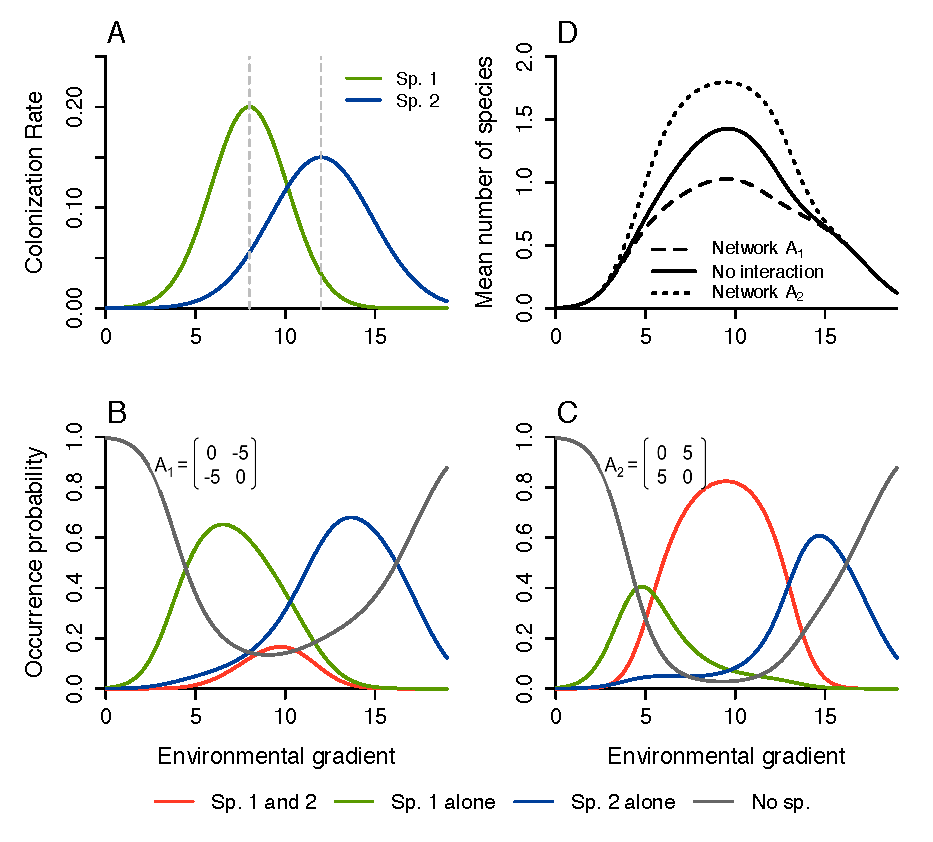
\includegraphics[width=0.8\textwidth]{./chapitre1/fig3.eps}
\caption[Equilibrium for interacting species along an environmental gradient]{\textbf{Equilibrium for interacting species along an environmental gradient}. The colonization probability of species $i$, $c_i$, is related to the environment variable $\mathbf{w}$ according to species-specific requirements (A). The intersection of the colonization curve of species $i$ with the grey dotted lines represents the value of $c_i$ associated with its environmental optimum $h_i$. We compute equilibrium occurrence probabilities for the different assemblages along the environmental gradient, for the networks $A_1$ with negative interactions (B) and $A_2$ with positive one (C). We calculate the expected species richness on the locality for the two networks and without interaction (D).
}
\label{chap1fig3}
\end{figure}



%--------------------------------------------------------------
\subsection{Biodiversity distribution over environmental gradients}

In this section, we introduce an environmental gradient to emphasize the interplay between interactions species-specific requirements along an environmental gradient. Our environmental gradient takes values from 0 to 30, for each of them we calculate the expected species richness associated to all scenario. To do so, we start by computing the colonization functions ($g_i$ functions): species optima $h_i$ are drawn from a uniform distribution from the range $[10,20]$ and the widths of the abiotic niches are kept constant for all the simulations $r_i=5$. Then we build the Markov chains for the different values of the environmental gradient and for the different $\mathbf{A}$ matrices. Again, we derive the vector $\mathbf{C_{eq}}$ and we sum its elements, i.e. occurrence probabilities of assemblage community, weighted by the species richness to which they refer. We repeat the procedure for an increasing value of connectance of $\mathbf{A}$ matrices: from 0 to 0.4. For this section, the parameter $d$ is set to 10, also extinction paramaters are set as follows: $e_i=10^{-5}$, $e_{i,min}=10^{-3}e_i$, $e_{i,max}=10^{3}e_i$ and $c_i=10^{-5}$. Like so we obtain the profile of species richness we report on Figure \ref{chap1fig5}.

For all scenarios, the richness is maximal at the center of the environmental gradient (Fig. \ref{chap1fig5}). This is due to the distribution of species optima in the range $[10,20]$. Also this is the range of environmental values for which the effect of interaction are the most important. Indeed, the higher the colonization probabilities, the higher interactions occur, therefore, interactions strongly impact species richness for favourable abiotic conditions. We also find that changes in species richness increase with connectance, as depicted by the colour of the solid lines for the three panels of Fig. \ref{chap1fig5}: from black (without interaction) to the lightest blue (connectance set to 0.4).

Species richness is inversely related to connectance when interactions are negative (Panel A in Fig. \ref{chap1fig5}). Moreover, when abiotic conditions are favourable, the number of species expected tends to 1. At the centre of the gradient, even though colonization probabilities are maximal, many species colonize but likely go extinct because of competition. We expect the locality to be most often occupied by species that are not affected by competition. Alternatively, in the case of positive interactions (Panel B in Fig. \ref{chap1fig5}), the expected species richness is strongly enhanced by interactions even for low connectance. The expected species richness tends to reach the total number of species from the most favourable to semi-harsh abiotic conditions. As the connectance increases the Gaussian shape of the richness profile turns into a hat shape, which has one major consequence: from favourable to semi-harsh conditions, the species richness is maintained thanks to positive interaction, but it also quickly collapses as the environment becomes slightly harsher.

Finally, when positive and negative interactions are mixed, the higher the connectance, the flatter the richness profile (Panel B in Fig. \ref{chap1fig5}). The expected species richness declines as connectance increases but far less than it does for negative interactions only. We think this is caused by the colonization of numerous prey that promote the survival of predators which in turn prevent assemblages to be as large as they can be without interaction (as predators reduce the persistence of prey). Conversely, from harsh to intermediate environmental conditions, mixed sign interactions positively affect the species richness. We explain this as the consequence of the benefit predators take from the preys presence. Assemblages with few predators, promoted by positive effect of the prey on their predators, may be relatively stable. Since colonization is low, this assemblage may enhance species richness over time but they may also collapse as soon as an extra predator colonizes the island.

%-------------------------
\begin{figure}[h!]
\centering
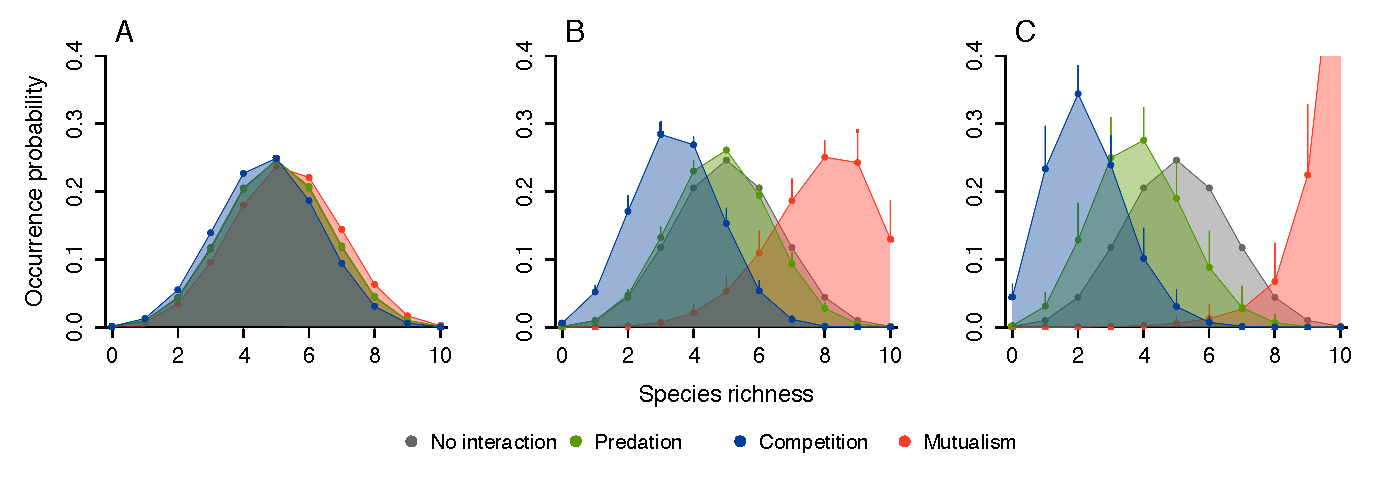
\includegraphics [width=\textwidth]{./chapitre1/fig4.eps}
\caption[Probabilities of species richness for different types of interaction]{\textbf{Probabilities of species richness for different types of interaction}. We compute expected species richness at the equilibrium with the following set of parameters: $e_i=10^{-5}$, $e_{i,min}=10^{-3}e_i$, $e_{i,max}=10^{3}e_i$ and $c_i=10^{-5}$. We do so for three different interaction weights: $d=0.1$ (A), $d=1$ (B), $d=10$ (C). In each panel, the four colours stand for the following types of networks: no interaction (grey), predation (green), competition (blue) and mutualism (red). Probabilities associated to coloured points are the means calculated for 1000 interaction matrices randomly-generated according to the niche model \citep{Williams2000} with a connectance set to 0.2. Additionally, vertical bars represent 50\% of the standard deviations associated to these means. To facilitate comparisons among panels, we do not represent the occurrence probability of the 10 assemblages community in panel C for mutualism, which is 0.66 (the standard deviation associated is 0.33).}
\label{chap1fig4}
\end{figure}





%--------------------------------------------------------------
\section{Discussion}

Understanding how colonization-extinction dynamics influence species distribution and community structure remains a major challenge in biogeography \citep{Wiens2011, Jabot2012, Godsoe2012}. Here, we build upon the simplicity of the Theory of Island Biogeography (TIB) to integrate crucial ecological processes, namely biotic and abiotic dimensions of the niche. Using the formalism of Markov chains, we derive an exact general solution for the occurrence probabilities of all possible assemblages that we calculate numerically (up to 10 species). Our approach is in stark contrast to the classic TIB \citep{MacArthur1967} where environmental gradients were not introduced and the co-occurrence among species was not modelled, despite empirical evidence of their impact \citep{Diamond1982}. By taking these constraints together we reveal how they interplay and affect species richness. We believe our approach offers new perspectives on the theory of biogeography and will support the development of species distribution models with the addition of species interactions.

%% i
In our model, we introduce the effect of biotic interactions as an ecological process affecting colonization/extinction probabilities. This has already been considered in many ways in the literature. For instance, more than forty years ago, Levins and Culver introduced extinction and migration rates affected by competition and showed analytically how it reduces co-occurrence \citep{Levins1971}. More recently, Jabot and Bascompte introduced production of eggs and seeds affected by interaction in an individual-based, meta-community framework and, hence, highlighted the potential effects of interactions on local diversity \citep{Jabot2012}. Also, Calcagno and colleagues demonstrated that tuning extinction and colonization rates based on the trophic relationships among species could explain the limited length of food chain \citep{Calcagno2011}. In contrast with previous studies, our approach is fully rooted on the TIB which yields well-defined null predictions (adding neither interaction nor environmental gradients), focuses on assemblages, and allows the investigation of the impact of any kind of network, including mixed interactions.

%-------------------------
\begin{figure}[h!]
\centering
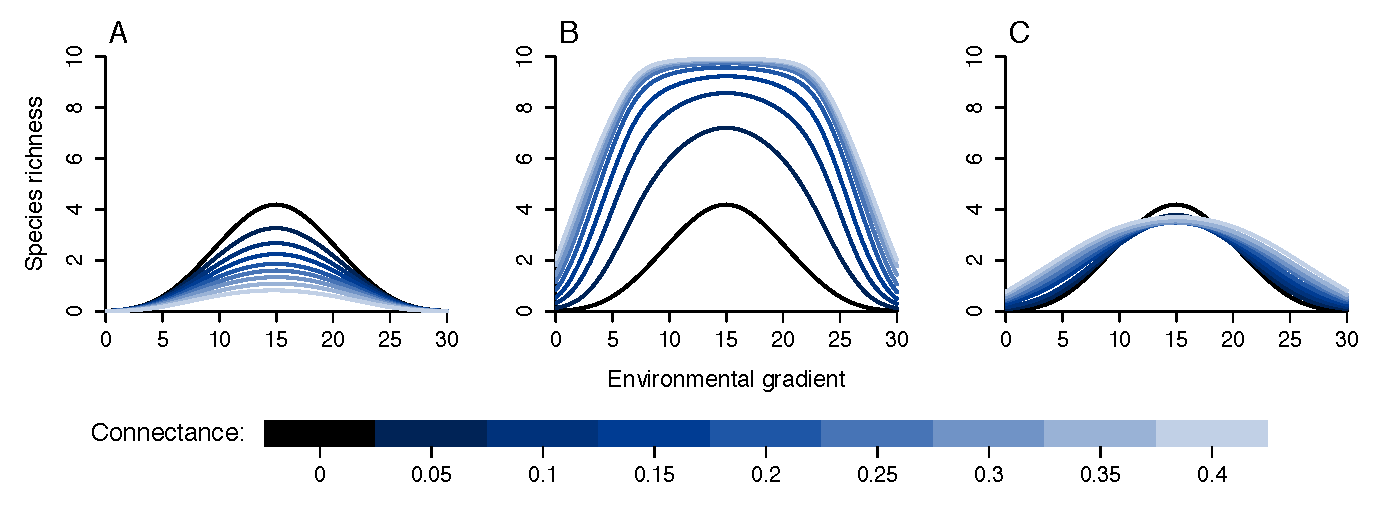
\includegraphics [width=\textwidth]{./chapitre1/fig5.eps}
\caption[Biodiversity distribution along environmental and connectance gradients]{\textbf{Biodiversity distribution along environmental and connectance gradients}. We compute the expected species richness along an environmental gradient for competition (A), mutualism (B) and predation (C). We do so for different values of connectance depicted by the shades of blue. Species richness profile associated with the scenario without interaction is provided in each panel by the darkest solid line (connectance set to 0). Abiotic niches do have the same range for all species ($r_i=5$) and the optima are randomly drawn in the interval $[10,20]$. The interaction weight ($d$) is set to 10. The extinction parameters are set as follows: $e_i=10^{-5}$, $e_{i,min}=10^{-3}e_i$, $e_{i,max}=10^{3}e_i$ and $c_i=10^{-5}$.}
\label{chap1fig5}
\end{figure}

Networks are convenient representations of the structure of ecological communities to study persistence and resilience \citep{Thebault2010}. A strength of our model is that it not only takes all direct interactions into account, but also indirect ones \citep{Wootton1994}. For instance, in a linear trophic chain of three species, the occurrence of the top predator depends not only on the presence of its prey but also on the species at the bottom of the chain \citep{Gravel2011}. This means that the distribution of the top predator will be influenced not only by its own abiotic requirements, but also by those of its prey and the species at the bottom of the chain. The signature of such indirect interactions should be common in co-occurrence networks. This property comes from the assumption that interactions change extinction rates and the Markov chain formalism employed. Our formalism therefore provides a tool, similar to the general Lotka-Volterra equations for the local scale, that could be used to study the emergence of indirect interactions in networks at the large spatial scale.

The challenge of developing joint species distribution models \citep{Pollock2014,Pellissier2013} have recently motivated researchers to investigate co-occurrence \citep{Araujo2014,Veech2013}.
Our framework helps to disentangle the two main processes by which non-random species associations (co-occurrence) can arise. First, two species not interacting with each other could be non-randomly co-distributed because of similar or antagonistic ecological requirements. As we introduced an abiotic constraint on the colonization probability, some assemblages will be more likely than others on a given environment simply because some species are favoured and others filtered out. We thus expect to find a signature of the covariance in species response to the environment on these assemblage probabilities. Secondly, non-random co-distribution will arise from ecological interactions. We considered an additive impact of all ecological interactions a species is experiencing from the community. Species interact in various ways, but at the end all interactions do impact demography by definition. This reality enters the model by either enhancing of decreasing extinction probabilities. In other words, the occurrence of a single species is derived from the expectation of observing all other species in the community.


%% ii
Our framework therefore provides a formalism to investigate the relationship between co-occurrence networks \citep{Araujo2011} and interaction networks. There is a significant amount of information contained in the data of co-occurrence, which is overlooked by most current methods of community analysis. Standard species distribution models are fitted to univariate presence/absence data, neglecting the information contained in the distribution of associated taxa. Multivariate statistics summarize the spatial structure of ecological communities, but they are essentially limited to the description of co-occurrence, they are not meant to predict species distributions conditional on other species. Most analyses of co-occurrence aggregate pairwise observations into a single index for the whole community, thereby missing substantial information pertaining to the consequences of biotic interactions \citep{Boulangeat2012}. This situation is not surprising given there is no general theory for co-occurrence. Current hypotheses are mostly limited to negative interactions, leading to negative co-occurrence (repulsion), or positive interactions, leading to positive co-occurrence (attraction). Many theoretical achievements are required to study co-occurrence for more complex assemblages, mixing positive, negative and antagonistic interactions. In addition, the impact of indirect interactions emerging in interaction networks on species distribution is ignored. Our approach provides a formal framework to overcome these limitations as we calculate assemblage probability at biogeographical scale and then derive co-occurrence. It also allows the decomposition of the strength of pairwise associations between abiotic and biotic drivers, opening the way for novel statistical developments of species distribution models taking into account this multi-occurrence information. We propose that studying the role of biotic factors at large scale requires us to introduce them as assemblages instead of adding species as factors which likely leads to non-equivocal conclusion \citep{Araujo2007}. In addition, our approach is not limited to species pairs, the assemblage probabilities provide a valuable tool to the co-occurrence of groups of species such as motifs \citep{Stouffer2007}.

The importance of interactions across different scales is still debated \citep{McGill2010,Araujo2014}. A common assumption is that interactions are negligible at large spatial scales, based on the rational that abiotic filters primarily determine the composition of assemblages \citep{Pearson2003}. This argument persists even though theoretical \citep{Gravel2011} and empirical \citep{Gotelli2010} evidence suggest the opposite. The key issue to solve this debate is thus to know how interactions can influence species assemblages with increasing spatial scale. Although the TIB still provide insights into the assembly of natural communities, the success of recent approaches integrating interactions strongly support their relevance at large scales. Indeed the addition of network structure \citep{Pellissier2013} or correlation between species \citep{Pollock2014} as proxies for interactions have adequately improved forecast accuracy. Here we do not solve this fundamental issue, however our model illustrates how species distribution at large scale will be impacted by the kind of interaction, their numbers and their distribution.

Although our framework is not readily applicable to real datasets, it nonetheless provides a theoretical foundation for the derivation of new statistical modelling approaches. We propose a different perspective which is rooted on theory, in contrast with what is usually done with phenomenological model representing the structure of the data \citep{Thuiller2013}. There are nonetheless significant challenges to apply our framework to empirical data. First, we must find a way to deal with large numbers of species. At present, given $n$ species in the regional pool, we compute an eigen vector of $2^n$ probabilities from a $2^n*2^n$ transition matrix of a Markov chain. Moreover, in its current formulation, it requires us to evaluate a very large amount of data including a description of network of the same species across time and space to get accurate estimations. Solving this issue will requires a rational to reduce the number of species considered. This could be achieved either by inference of the relevant interactions, or alternatively by pooling species into groups. A systematic and rigorous method to build meaningful groups of interacting species from proxies such as traits and phylogenies remains to be developed, but there are nonetheless promising avenues \citep{Baskerville2011}. The relatively small number (from 3 to 7) of dimensions to ecological networks, i.e. the number of trait-axes required to properly infer interactions \citep{Eklof2013}, supports its feasibility. A second challenge is to account for spatial structure that constrains population flux. Despite the theoretical developments, applied approaches to model species distribution struggle to introduce it efficiently \citep{Boulangeat2012}. The island-mainland approximation remains elegant but might be too simple for applied situations. One solution may be to identify source and sink localities, \citep{Boulangeat2012}. This requires us to consider i) species abundances and ii) spatial structures which would strongly increase the complexity of the model. One first step forward could be to apply the Levins model rather than the island-mainland model as Levins and Culver did to study the impact of competition \citep{Levins1971}.

%% iii
Despite our call for a new integrated theory of biogeography, we acknowledge the limitations of the framework. Recent studies aimed at integrating population dynamics, for instance, using approximations from the metabolic theory of ecology. This is a hopeful direction to assess local extinction risk, accounting for network structure, body size and abundance \citep{Schneider2012}. Beyond body size, other functional traits \citep{McGill2006} could help us to escape from species singularity toward more general rules. Hence, approximating food web structure could be done using traits \citep{Gravel2013} and energetic requirements can be easily quantified through body size and local temperature constraints \citep{Brown2004}. Moreover considering changes in traits over time may be a key to introduce evolutionary processes. This would help us to release one strong assumption of our work: no speciation processes are taken into account. Although it might not matter for short time periods, having a pool of species unchanged becomes a major issue for time scales that exceed by far the lifespans of species we consider. Further, our framework could be applied to investigate diversification dynamics on remote areas, with a particular emphasis on the effect of ecological interactions on adaptive radiations. Despite the complexity of such model, it would very likely provide valuable insights on the future of biodiversity under current global change.

Since the seminal work of Davis et al. \citep{Davis1998}, there is growing evidence that the response of species to climate change must be studied at the community scale \citep{Suttle2007}. Even though species respond individually to climate change, they are constrained by complex direct and indirect biotic interactions emerging from large scale organization \citep{Lavergne2010}. The study of Cahill and colleagues \citep{Cahill2013} has revealed the difficulties to link climate changes and species extinction. Even when the climate is expected to drive local extinctions, it actually implies a chain of perturbations amidst which biotic factors prevail \citep[\emph{e.g.} loss of prey][]{Durance2010}. For instance, species contributing to the persistence of plant-pollinator networks are paradoxically the most vulnerable to extinction \citep{Saavedra2011}, highlighting the risk of extinction cascades. As S\"aterberg et al. expressed, ``the species to be the first to go extinct is not the one whose mortality rate is increased but instead some other species in the food web'', thereby suggesting that perturbations which affect species differently also spread over the network making extinction difficult to predict \citep{Saterberg2013}. Although this is fully understandable as species interact, this makes forecasting of future species distributions more complicated. Therefore the challenge of proposing biodiversity scenarios to global change requires new approaches integrating ecological processes over time and spatial scales, and to disentangle their relative contribution \citep{Lavergne2010}. We think that the assemblage-based approach we propose here is a promising perspective to introduce interactions in biogeographical models.


%--------------------------------------------------------------
\section{Acknowledgment}
We thank Chantal L. Hutchison for insightful comments on the manuscript.
KC was supported by a grant from the Ministry of Higher Education and Research of France. DG was supported by a NSERC Discovery grant and the Canadian Research Chair program. NM was supported by the CNRS.
